\documentclass{article}
\usepackage{graphicx} % Required for inserting images
\usepackage[smartEllipses]{markdown}
\usepackage[left=2cm,right=2cm,top=2cm,bottom=2cm]{geometry} % Adjust margins as needed
\usepackage{array}
\usepackage{makecell}

%Task and support template

%\begin{table}[htbp]
%    \centering
%    \begin{tabular}{|p{5cm}|p{10cm}|}
%        \hline
%        \multicolumn{2}{|c|}{\makecell[cl]{\textbf{Task:} \\
%        \textbf{Purpose:} \\
%        \textbf{Frequency:}}}\\
%        \hline
%        % Row 1
%        Sub task 1 & Example Solution 1 \\
%        \hline
%        % Row 2
%        ? & ? \\
%        \hline
%        % Row 3
%        ? & ? \\
%        \hline
%        % Row 4
%        ? & ? \\
%        \hline
%        \multicolumn{2}{|c|}{\makecell[cl]{\textbf{Variant:}}}\\
%        \hline
%        ? & ? \\
%        \hline
%    \end{tabular}
%    \caption{Example Table}
%    \label{tab:example}
%\end{table}



\title{Software Requirements Specification
Document\\
Cosy Koala IT}

\author{
  Vincent, Malzinskas\\
  \texttt{6474322}
  \and
  Aashim Lal, Memanaparambil Asokalal\\
  \texttt{103794571}
  \and
  Jordan, Zaz\\
  \texttt{6386601}
  \and
  Julian, Lai\\
  \texttt{103594920}
}

\date{March 2024}

\begin{document}

\maketitle
\newpage
\tableofcontents
\newpage


\section{Introduction}
This document contains the specifications for a operational information system (OIS) for the Cosy Koala restaurant in Hawthorn Vic. This document will outline the specifications, requirement and quality attributes of the operational information system

\subsection{Purpose}
The purpose of this document is to detail the functionalities and features of the OIS, aiming to streamline various restaurant operations as the business grows. From customer management and interactions to internal services and task management, the goal of this system is to allow the Cosy Koala to operate at a targeted customer patronage of 150 guests.

\subsection{Scope}
The OIS will facilitate the following high level tasks:
\begin{enumerate}
    \item Customer Management.
    \item Customer Interaction.
    \item Internal Services.
\end{enumerate}


\section{Project Overview}
The Cosy Koala currently sits 50 customers. It is making a physical expansion on premises to sit 150 customers. The current technical integration with operations is low. Taking orders from guest and interacting with the kitchen, and accounting is handled by hand.
The Cosy Koala has identified multiple ideas they would like to include in the OIS:
\begin{enumerate}
    \item The new system shall support reservations.
    \item The new system shall support taking orders from customers.
    \item The new system shall support information sharing with the Kitchen.
    \item The new system shall support creating invoices.
    \item The new system shall support creating receipts for customers.
    \item The new system shall support handling payments.
    \item The new system shall support basic statistics about ordered menu items.
    \item The new system shall support online availability of the menu.
    \item The new system shall support ordering from online take-away menus.
    \item The new system shall possibly support arranging delivery.
\end{enumerate}

\subsection{Domain Vocabulary}
\begin{enumerate}
    \item OIS : Operation Information System.
\end{enumerate}
\subsection{Pain Points}
\begin{enumerate}
    \item Customer information:
    \begin{enumerate}
        \item Managing 50+ customer orders.
        \item Taking onsite orders.
        \item Taking offsite orders.
        \item Collecting data on sales.
        \end{enumerate}
    \item Front to back of house interactions:
    \begin{enumerate}
        \item Organize orders.
        \item Make sure food is sent to correct customer.
    \end{enumerate}
    \item Administrative functions:
    \begin{enumerate}
        \item Gather customer data.
        \item Update website with marketing data.
        \item Analyse customer data.
        \item Provide offsite order and payment.
        \item Provide delivery.
    \end{enumerate}
\end{enumerate}


\subsection{Domain Entities}
\begin{enumerate}
    \item Meal
    \item Payments
    \item Customer
    \item Front of House Staff
    \item Table
    \item Dining Room
    \item Receipts
    \item Sales Data
    \item Order
    \item Marketing Data, i.e. Menu lists, JPGs etc.
    \item Point of Sales
\end{enumerate}


\subsection{Actors}
\begin{enumerate}
    \item Onsite Customer
    \item Offsite Customer
    \item Front of House Staff Member
    \item Back of House Staff Member
    \item Admin
    \item Website
    \item Delivery System
\end{enumerate}

\subsection{Task - Brief}
\begin{enumerate}
    \item Take onsite customer order .
    \item Take offsite customer order.
    \item Take onsite customer payment.
    \item Take offsite customer payment.
    \item Create offsite customer receipt.
    \item Create onsite customer receipt.
    \item Communicate order with Kitchen.
    \item Seat customer.
    \item Drop food to customer.
    \item Deliver food to customer.
\end{enumerate}


\subsection{Project Goals \normalsize\textbf{Author: Vincent}}
\subsubsection{Primary Goals}
The primary Goal of Cosy Koala and the reason for releasing a tender for an OIS software provider is to be able to support a physical increase of guest from 50 to 150 in their restaurant.
\subsubsection{Secondary Goals}
\begin{enumerate}
    \item Support increased business through take-away.
    \item Support informed customers through their website.
    \item Support informed management about the customers purchases.
    \item Capture potential customers through their website.
\end{enumerate}
\subsubsection{Tertiary Goals}
Cosy Koala is interested in the possibility of supporting the arrangement of delivery.

\subsection{Assumptions \normalsize\textbf{Author: Vincent}}
A number of assumptions are made in relation to the implementation of this OIS is that manual scaling of operations are impossible. Whether that means no more staff will be available. Or whether staff will be expected to have other duties.


\clearpage

\section{Problem Domain}

\subsection{Data model \normalsize\textbf{Author: Vincent}}

\clearpage
\subsubsection{Domain model \normalsize\textbf{Author: Vincent}}
\begin{figure}[!h]
    \centering
    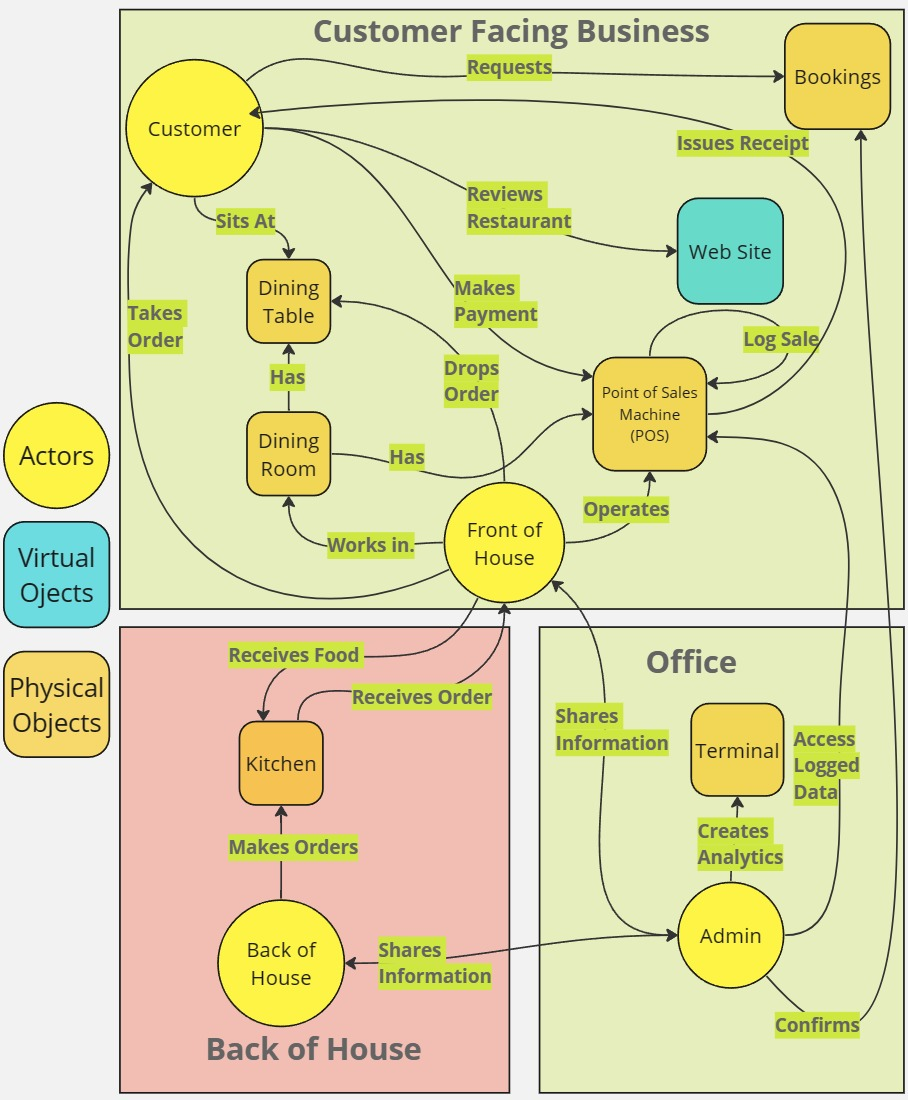
\includegraphics[width=15cm]{Domain_Model.jpg}
    \caption{Cosy Koala Domain Model}
    \label{fig:Domain_Model}
\end{figure}
\subsubsection{Entity Descriptions}
Customer: Is a person dining on food or beverages prepared by Cosy Koala. This can be on site or take away (TA).\\\\
Front of House: This is a staff member who has direct contact with the customer. They take orders from customers. Take orders to the Kitchen. Bring customers their food. They are responsible for maintaining the orders integrity (Making sure the customer gets what they pay for). The take customer transactions. Communicate with Admin.\\\\
Back of House: Prepare the customers food order. Responsible for making sure front of house receive the food order with correct information i.e. order number etc. Communicate with Admin.\\\\
Admin: Get the logged data from the Point of Sales Machine.
Generate analytics from the Sales data.
Web Site: Display general information about the restaurant.\\\\
Dining Room: Containerizes and organizes customers orders i.e. If the restaurant has a multiple rooms this can be used to better locate customers for orders.\\\\
Dining Table: Creates a sub container for organizing customers orders.\\\\
Point of Sales Machine: Facilitates payment transactions. Issues receipts.\\ Logs sales data. Is operated be a front of house staff member.
Kitchen: Containerizes and organizes customers food order for pick up.\\\\
Terminal: Allows for the manipulation and reading of logged Sales Data.\\\\

\subsection{Tasks}

\subsection{}
\begin{table}[htbp]
    \centering
    \begin{tabular}{|p{5cm}|p{10cm}|}
        \hline
        \multicolumn{2}{|c|}{\makecell[cl]{\textbf{Task:} Complete Payment transaction onsite. \\
        \textbf{Purpose:} Take the money owed to the restaurant after a sale of a food or drink and issue receipt.\\
        \textbf{Frequency:} Up to 150 times a breakfast, lunch or dinner service.}}\\
        \hline
        % Row 1
        \textbf{Sub task 1} & \textbf{Example Solution 1} \\
        \hline
        % Row 2
        Locate the meal in system. & Enter the table number, and dining room name in order to find the meal. \\
        \hline
        % Row 3
        Inform customer of details of meal, price etc. & The GUI can display relevant meal information. \\
        \hline
        % Row 4
        Initiate payment system. & FoH Staff member can send the price of the meal to the EFTPOS machine. \\
        \hline
        % Row 5
        Display whether the payment was successful. & The GUI can display to the customer and the staff member whether payment was successful. \\
        \hline
        % Row 6
        Offer to print receipt. & The GUI could display an option for the FoH or Customer to select to print a receipt. \\
        \hline
        Print receipt & System send information to printer, possibly by network. \\
        \hline
        Move transaction to new state - payed & The system can validate the transaction was successful and move the meal to a payed/cleared data storage. \\
        \hline
        \multicolumn{2}{|c|}{\makecell[cl]{\textbf{Variant:}}}\\
        \hline
        Customer only wants to pay for their meal and a table with multiple people & System should allow the FoH to select items from a meal for individual payment. \\
        \hline
    \end{tabular}
    \caption{Taking Payment}
    \label{tab:example}
\end{table}

\subsection{}
\begin{table}[htbp]
    \centering
    \begin{tabular}{|p{5cm}|p{10cm}|}
        \hline
        \multicolumn{2}{|c|}{\makecell[cl]{\textbf{Task:} \\
        \textbf{Purpose:} \\
        \textbf{Frequency:}}}\\
        \hline
        % Row 1
        Sub task 1 & Example Solution 1 \\
        \hline
        % Row 2
        ? & ? \\
        \hline
        % Row 3
        ? & ? \\
        \hline
        % Row 4
        ? & ? \\
        \hline
        \multicolumn{2}{|c|}{\makecell[cl]{\textbf{Variant:}}}\\
        \hline
        ? & ? \\
        \hline
    \end{tabular}
    \caption{Example Table}
    \label{tab:example}
\end{table}


\subsection{Workflows \normalsize\textbf{Author: Vincent}}
\subsubsection{}


\subsection{Functional Requirements and Task Descriptions}
\begin{figure}[!h]
    \centering
    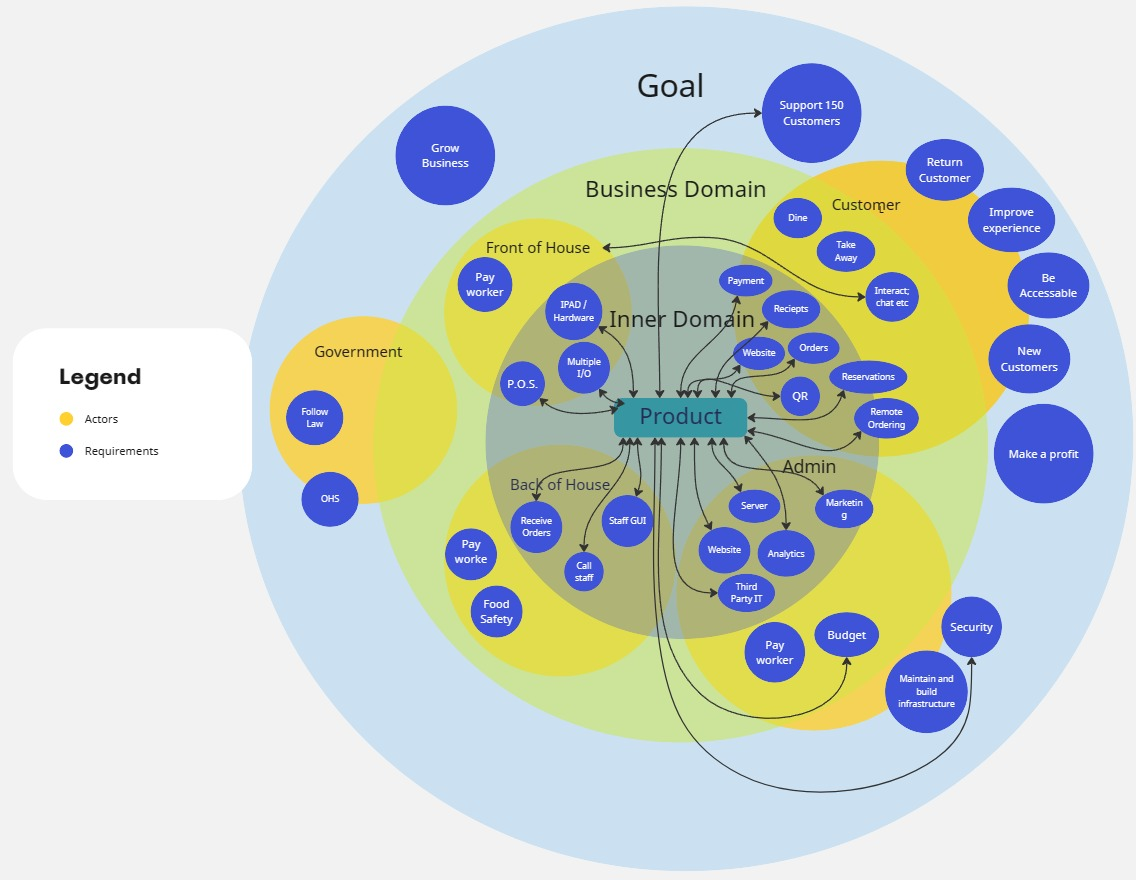
\includegraphics[width=15cm]{Domain_product_diagram.jpg}
    \caption{Cosy Koala Domain Requirements}
    \label{fig:Domain_Product}
\end{figure}

\section{Quality Attributes of System}
\section{Other Requirements}
\section{Validation of Requirements}
\section{Possible Solutions}


\end{document}
